%!TEX root = ../main.tex

\section{Results from CDB optimization} % (fold)
\label{sec:cdb_optimization}

%We now consider the relative diversification benefit of HML, CMA and RMW. We study the evolution of optimal CDB over time for different five- and six-factor universes, and experiment with the exclusion of one of HML, CMA and RMW at a time. The intuition behind this exercise is to see how much diversification is lost if we can no longer invest in a given factor. Does excluding HML make the portfolio less diversified than excluding CMA? And what is the impact of the other new factor, RMW? 

We begin by comparing the optimal CDB weights to the optimal MV weights in \autoref{fig:cdb_mv_compare}.\footnote{The graphs excluding one factor at a time are still made available in \autoref{app:cdb_weights}.} The difference between weights under CDB and MV optimization are found to be fairly small -- especially for Mkt.RF, and to a lesser extent for HML and CMA.  It rather seems that the CDB optimal weights are less erratic in their pattern, which is likely to be due to the fact that MV optimization takes into consideration the conditional expected return, while CDB optimization only concerns tail risk. The most notable difference between CDB and MV weights is that CDB seems to allocate less into Mom. Again, this is coherent, as the CDB optimization does not reward the factor for its high expected return. 

Next, we study the CDB over time with CDB optimized weights, where we experiment with excluding one of the factor HML, CMA and RMW at a time. The results are given in \autoref{fig:cdb_cdb}, and are based on a Value-at-Risk cut-off of 5\%.\footnote{In unreported results, the lower cut-off values of 1\% is found to be qualitatively similar.} We proceed with a number of interesting results that emerge from this picture:

% CDB is very high; factor strategies are good diversifiers
First, we note that regardless of whether momentum is included or not, factor strategies appear to offer high levels of diversification. In absolute terms, all strategies fluctuate in the 80--95 range for the majority of the studied time period. 

% Dips
Second, there are notable dips in the diversification benefit measure. The dips represent times when diversification is relatively hard to come by, and roughly coincide in the five- and six-factor models. Interestingly, the periods of low diversification do not seem be stock market crises, as the CDB measure remains relatively high during the 1999-2000 bubble and the 2007-2009 recession [if we are using these names elsewhere, we need a convention for their naming and year breaks].

% HML is a better diversifier on average
% CMA better when diversification is hard to come by
Third, the level decreases in diversification benefit of removing HML or CMA seem quite small. Furthermore, this decrease is highly similar; At certain times, portfolios including HML are more diversified and vice versa, but no pattern emerges. However, we note that the exclusion of RMW is dramatically different. Without RMW, the level decrease is substantial and dips in CDB become much more pronounced and frequent. 

For comparison, we also report the CDB over time with MV optimized weights in \autoref{fig:mv_cdb}. This allows us to study how well tail diversified an MV portfolio is. In comparison to the optimal CDB in \autoref{fig:cdb_cdb}, we note that the MV optimization leads to considerably lower tail diversification. Changing to MV optimization leads to a level shift as well as more frequent and deeper dips. Interestingly, the change to MV weights makes diversification benefits worse especially for the model where RMW is excluded. We find it interesting for MV oriented factor investors that including RMW significantly limits the tail risk in MV portfolios. In a number of periods, incl. 1972-1974, 1976-1978, 1980-1982, and 1990-1993, a number of severe declines in tail diversification are avoided almost entirely if RMW is included. 

\begin{figure}[htbp]
  \centering
  \footnotesize
  \begin{subfigure}{0.45\textwidth}
    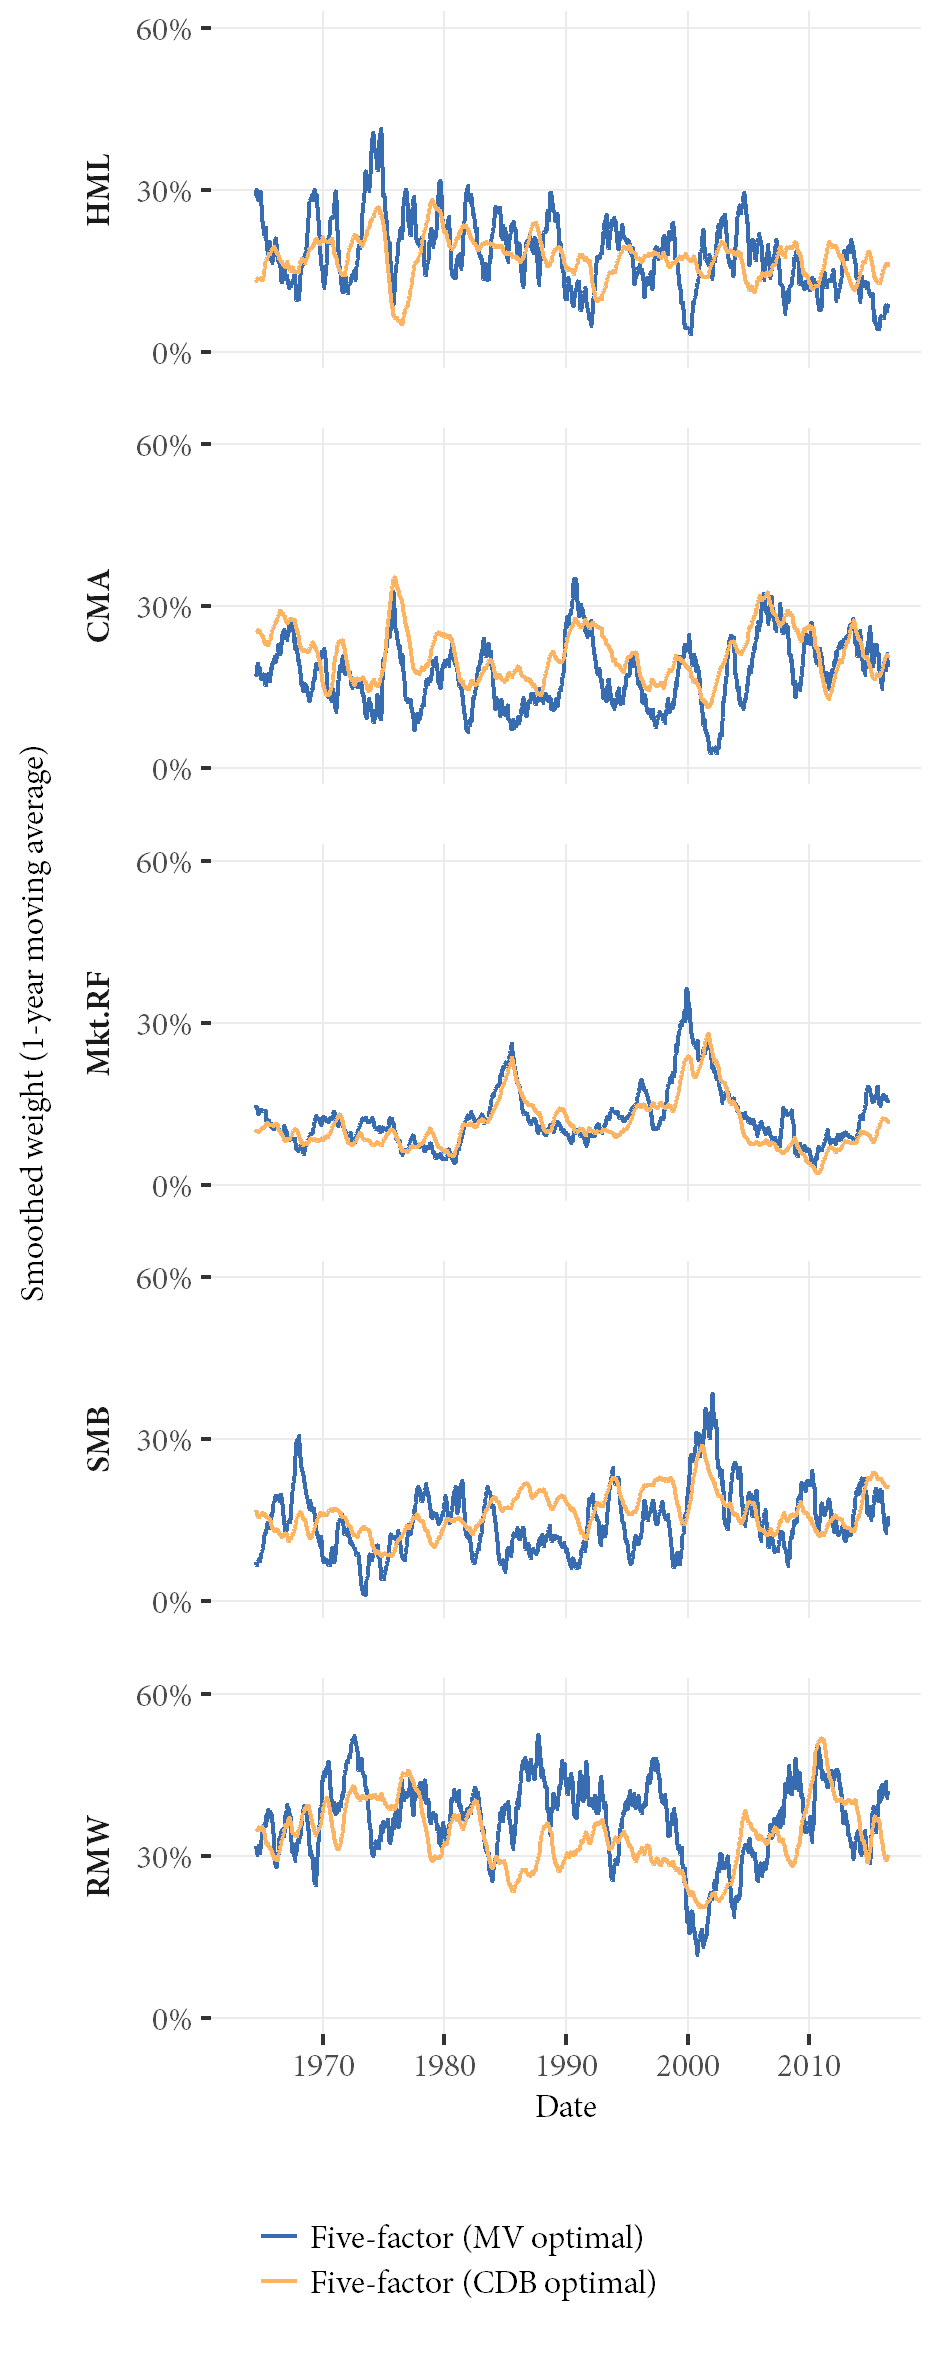
\includegraphics[width=\textwidth]{graphics/weights/compare_Weights_CDB_MV_5F.png}
    \caption{Five-factor universe}
  \end{subfigure}
  ~
  \begin{subfigure}{0.45\textwidth}
    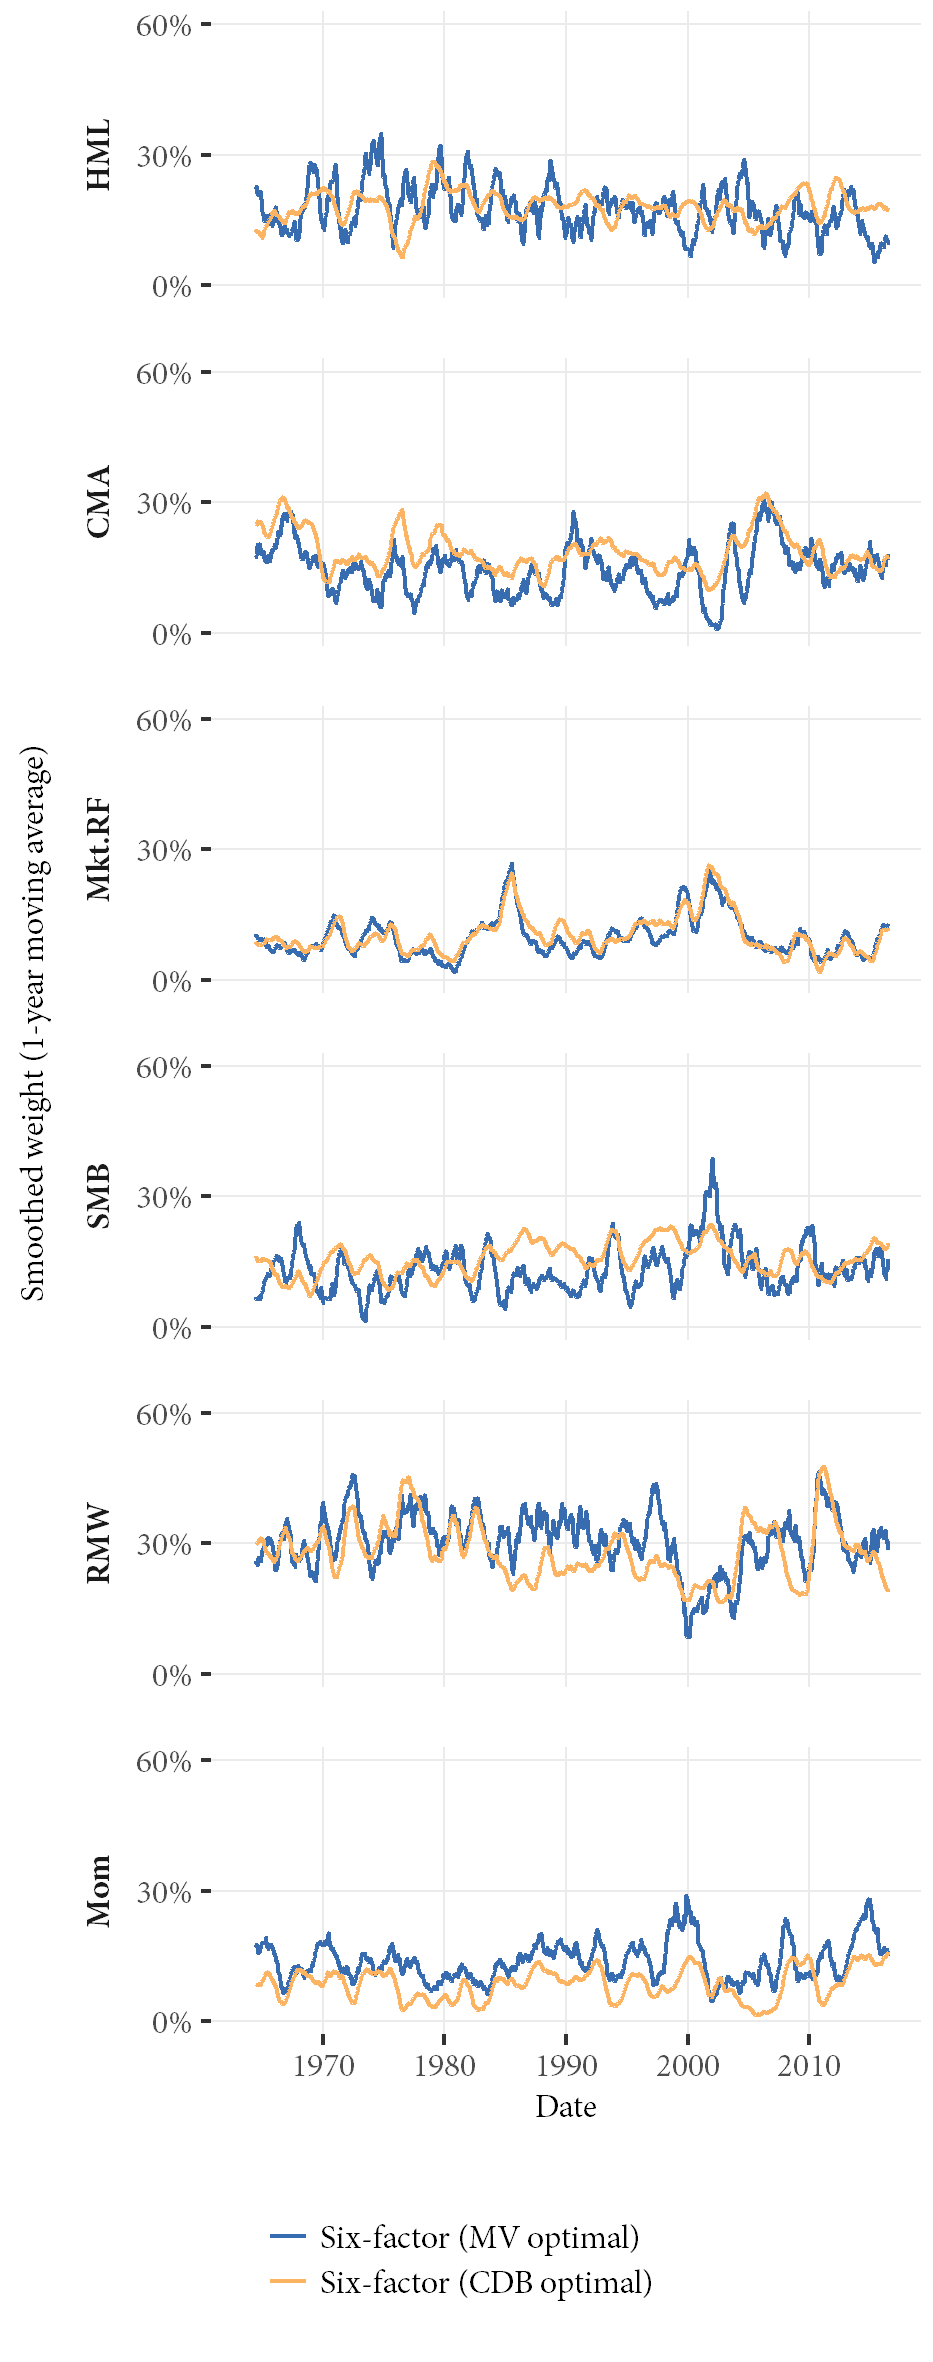
\includegraphics[width=\textwidth]{graphics/weights/compare_Weights_CDB_MV_6F.png}
    \caption{Six-factor universe}
  \end{subfigure}  
  \caption{Comparison of CDB optimal weights and MV optimal weights}
  \label{fig:cdb_mv_compare}

  \begin{longcaption}
    Smoothed as 1-year moving averages. Based on one-week-ahead forecasts from the copula model 1963--2016.
  \end{longcaption}
\end{figure}

\begin{figure}[!ht]
  \centering
  \footnotesize
  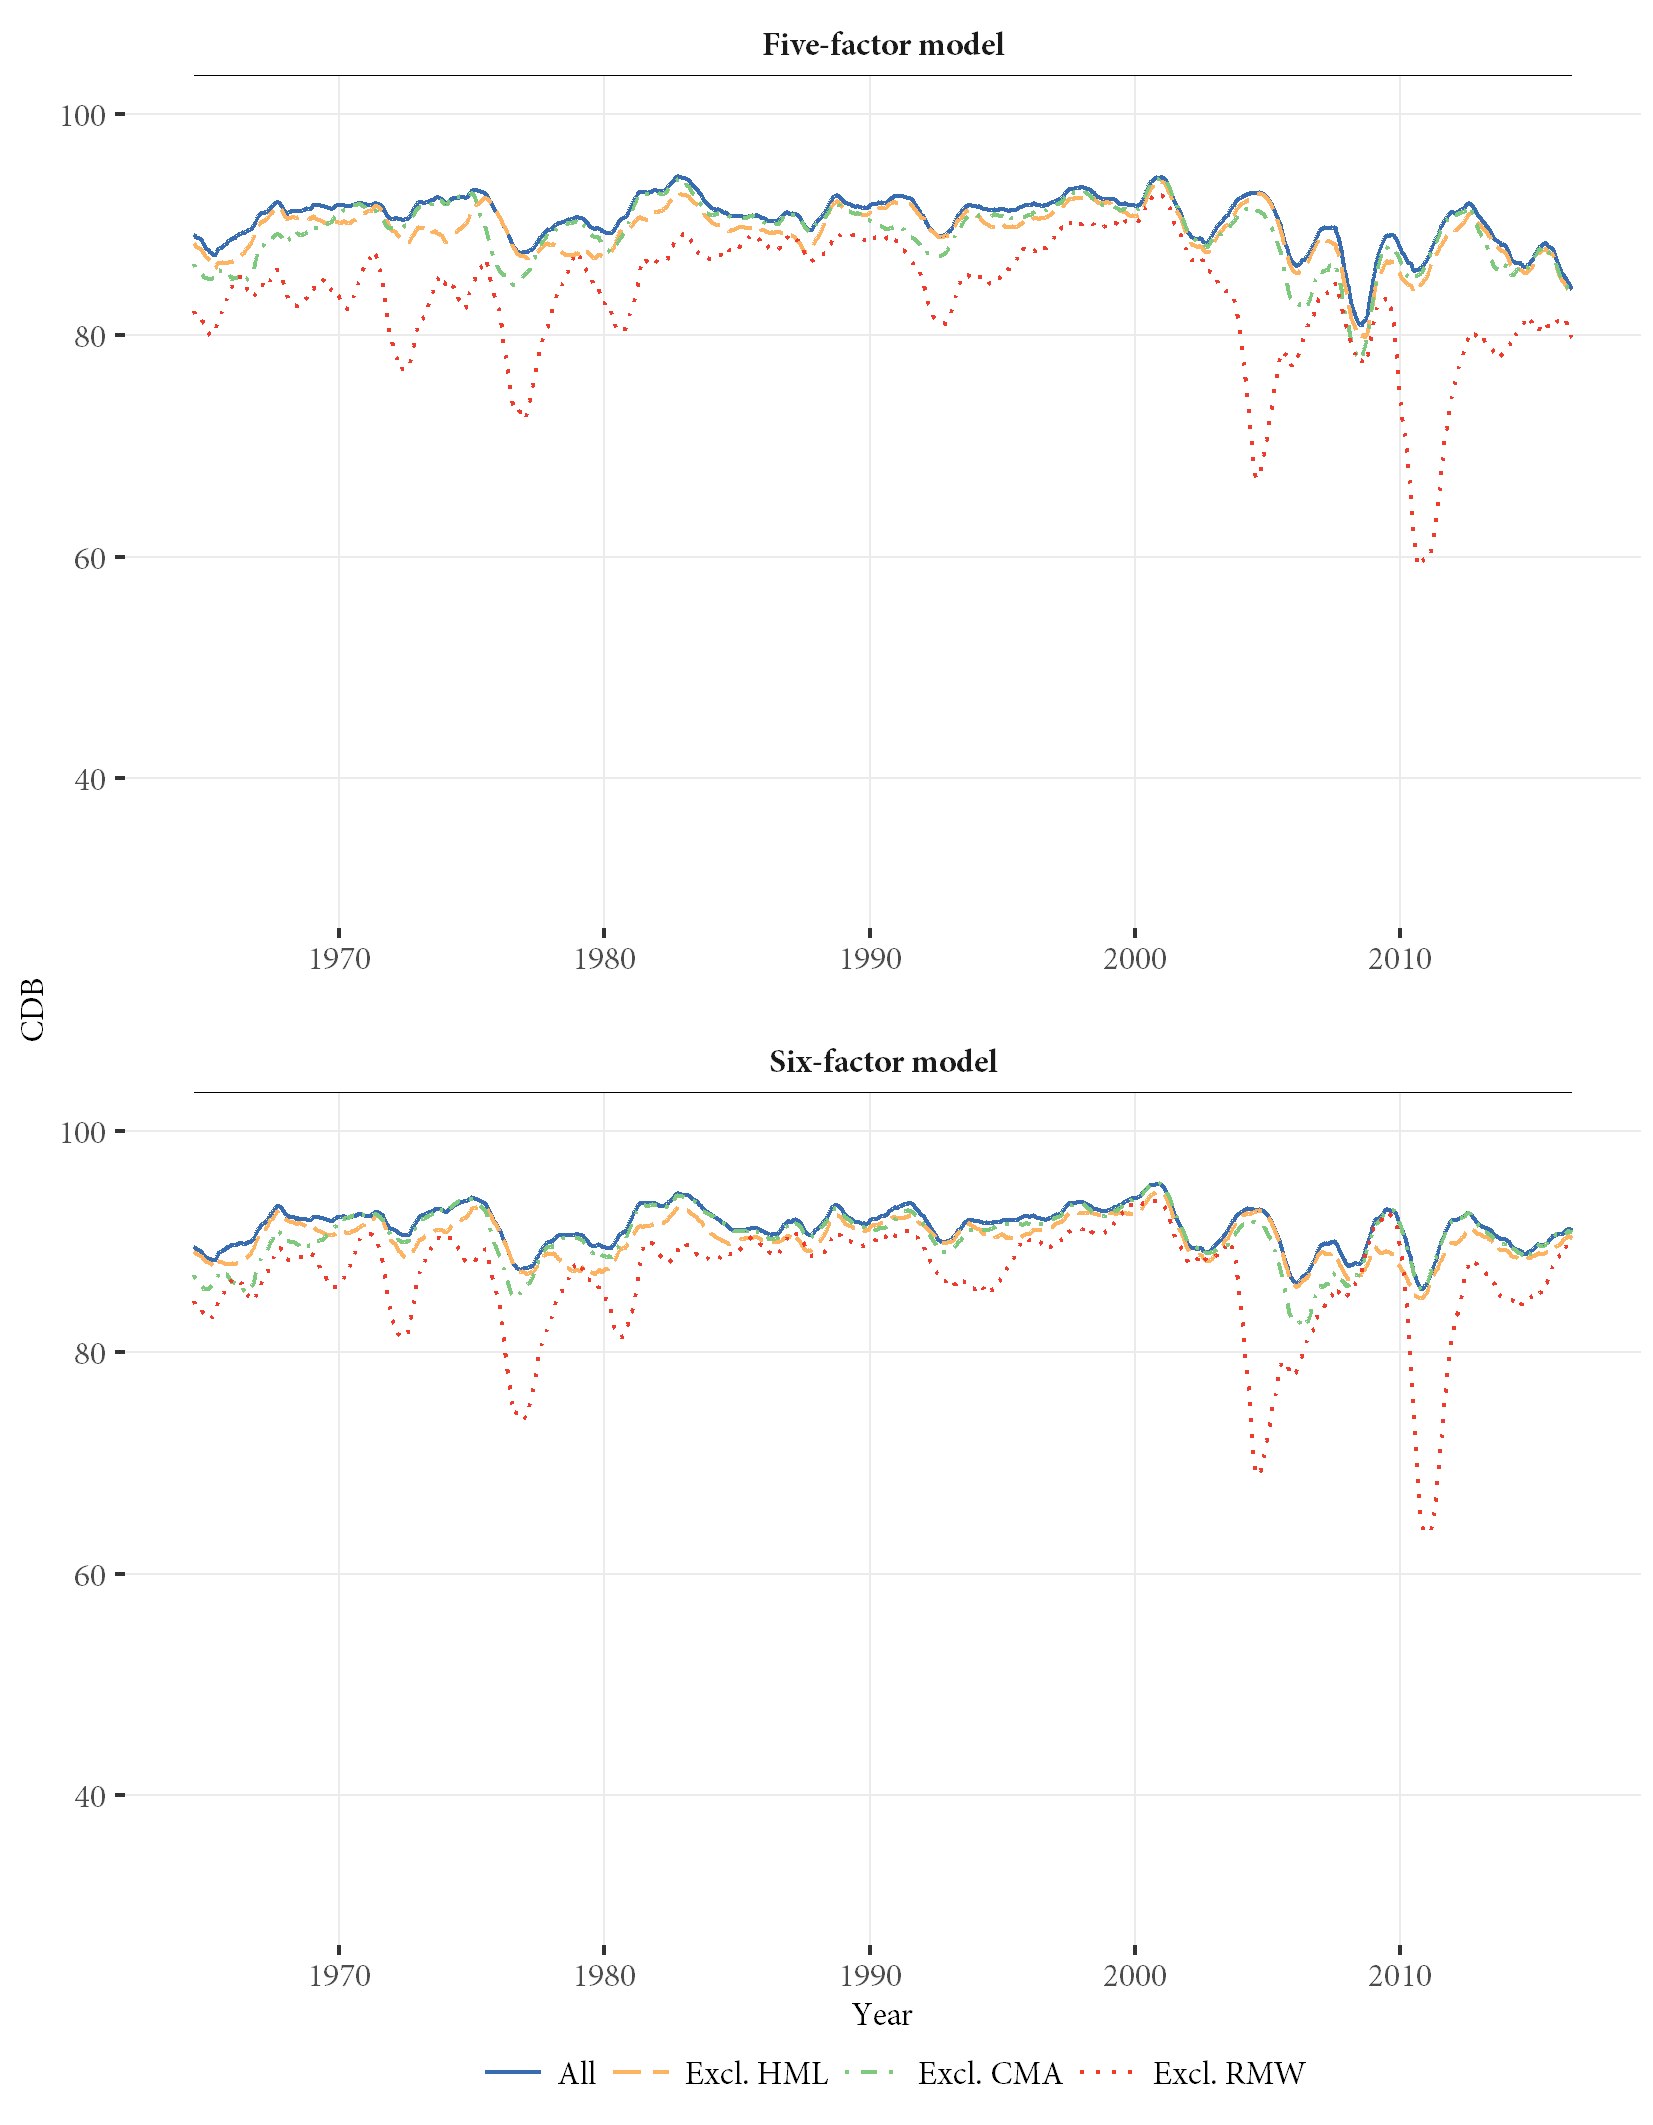
\includegraphics[width = \textwidth]{graphics/cdb/CDB.png}
  \caption{5\% Conditional Diversification Benefit (CDB) for CDB optimal weights}

  \begin{longcaption}
    Five- (without Momentum) and six-factor universes. The line has been smoothed with a moving average on a quarterly window to make it easier to read. See \autoref{sub:conditional_diversification_benefit} for computational details.
  \end{longcaption}
  \label{fig:cdb_cdb}
\end{figure}

\begin{figure}[ht!]
  \centering
  \footnotesize
  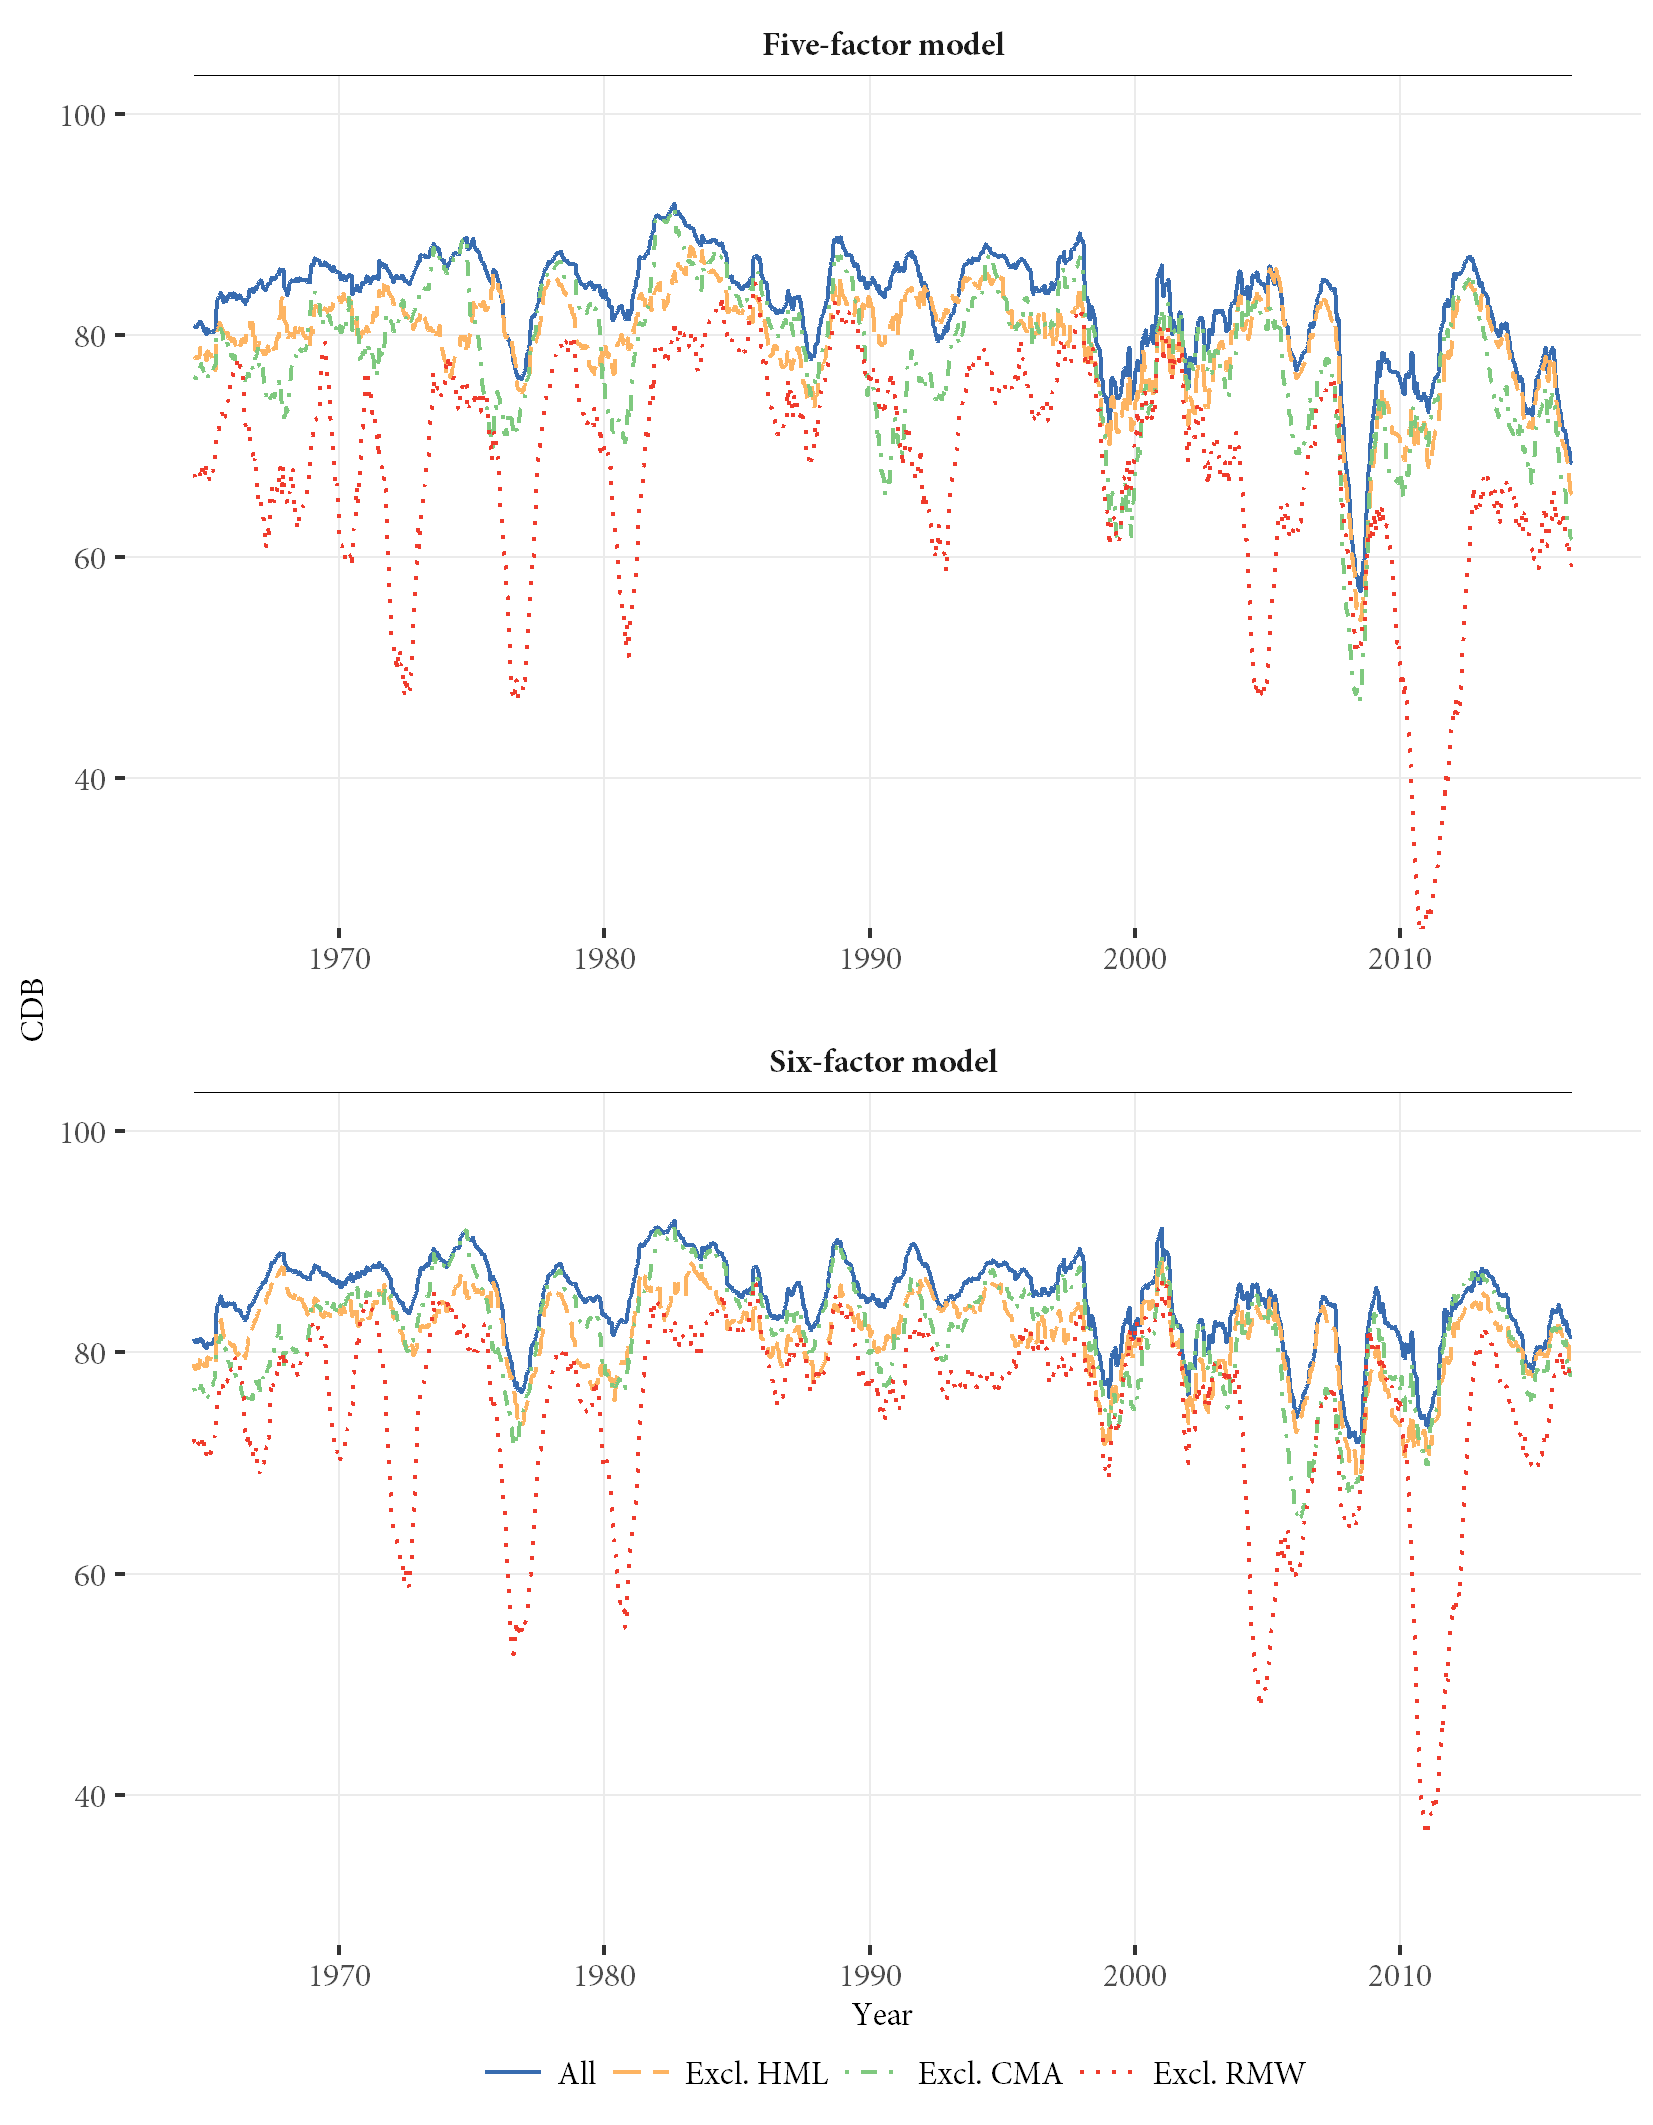
\includegraphics[width=\textwidth]{graphics/cdb/MV.png}
  \caption{5\% Conditional Diversification Benefit (CDB) for MV optimal weights}

  \begin{longcaption}
    Five- (without Momentum) and six-factor universes. The line has been smoothed with a moving average on a quarterly window to make it easier to read. See \autoref{sub:conditional_diversification_benefit} for computational details.
  \end{longcaption}
  \label{fig:mv_cdb}
\end{figure}

%!TEX root = ../../main.tex

\begin{table}
  \centering
  \footnotesize
  \renewcommand{\arraystretch}{1.2}

  \caption{CDB optimization with dynamic copula model (1963--2016)}

  \begin{longcaption}
    Average weights are averages of dynamic CDB optimal weights based on simulations of the return distribution from the dynamic symmetric \emph{t} copula model. Differences in average weights are expressed relative to the full five- and six-factor models. Performance measures are based on realized returns. SR is the annualized Sharpe Ratio. VaR, ES and CDB are all based on the one-week-ahead 5\% lower tail of the return distribution. Differences in CDB are to be read as column model minus row model and its associated standard errors (in parentheses) are computed taking the copula model as given.
  \end{longcaption}

  \label{tab:cdb_model}

  \begin{tabularx}{\textwidth}{@{} l dddd X dddd @{}}
    \toprule
    &
      \multicolumn{4}{c}{Five (four) factor models} &&
      \multicolumn{4}{c}{Six (five) factor models} \\
    \cmidrule{2-5}
    \cmidrule{7-10}
    &
      \multirow{2}{*}{All} &
      \multicolumn{1}{c}{Excl.} &
      \multicolumn{1}{c}{Excl.} &
      \multicolumn{1}{c}{Excl.} & &
      \multirow{2}{*}{All} &
      \multicolumn{1}{c}{Excl.} &
      \multicolumn{1}{c}{Excl.} &
      \multicolumn{1}{c}{Excl.} \\
    &
      &
      \multicolumn{1}{c}{HML} &
      \multicolumn{1}{c}{CMA} &
      \multicolumn{1}{c}{RMW} &&
      &
      \multicolumn{1}{c}{HML} &
      \multicolumn{1}{c}{CMA} &
      \multicolumn{1}{c}{RMW} \\
    \midrule
    \multicolumn{1}{@{}l}{\textbf{Average weights}} \\
    Mkt.RF & 11.1 & 10.5 & 11.5 & 19.2 & & 10.5 & 10.1  & 10.6 & 15.5 \\
    SMB    & 16.6 & 18.3 & 19.1 & 22.6 & & 15.8 & 17.9 & 18.1 & 19.2 \\
    HML    & 17.4 &      & 30.1 & 26.7 & & 18.1 &      & 28.7 & 24.9 \\
    CMA    & 21.2 & 35.0 &      & 31.6 & & 18.7 & 32.2 &      & 24.1 \\
    RMW    & 33.8 & 36.2 & 39.3 &      & & 28.1 & 31.8 & 32.6 & \\
    Mom    &      &      &      &      & &  8.8 & 8.1  & 10.0 & 16.2 \\
    \midrule
    \multicolumn{1}{@{}l}{\textbf{Difference weights}} \\
    Mkt.RF & & -0.6  & 0.4   & 8.1   & & & -0.4  & 0.2   & 5.1 \\
    SMB    & & 1.7   & 2.5   & 6.0   & & & 2.1   & 2.3   & 3.4 \\
    HML    & & -17.4 & 12.7  & 9.3   & & & -18.1 & 10.6  & 6.8 \\
    CMA    & & 13.9  & -21.2 & 10.4  & & & 13.5  & -18.7 & 5.4 \\
    RMW    & & 2.4   & 5.5   & -33.8 & & & 3.7   & 4.4   & -28.1     \\
    Mom    & &       &       &       & & & -0.7  & 1.3   & 7.5 \\
    \midrule
    \multicolumn{1}{@{}l}{\textbf{Performance}} \\
    Mean (\%)      & 2.77  & 2.94  & 2.85  & 3.37  & & 3.37  & 3.39  & 3.41  & 3.90 \\
    SD (\%)        & 2.42  & 2.49  & 2.69  & 3.89  & & 2.37  & 2.52  & 2.56  & 3.49 \\
    SR             & 1.14  & 1.18  & 1.06  & 0.87  & & 1.42  & 1.34  & 1.33  & 1.12 \\
    Avg. VaR  (\%) & 0.46  & 0.48  & 0.52  & 0.78  & & 0.45  & 0.47  & 0.49  & 0.69 \\
    Avg. ES  (\%)  & 0.61  & 0.64  & 0.69  & 1.04  & & 0.60  & 0.64  & 0.66  & 0.92 \\
    Avg. CDB       & 90.42 & 89.29 & 89.19 & 83.42 & & 91.33 & 90.24 & 90.51 & 86.62 \\
    \midrule
    \multicolumn{1}{@{}l}{\textbf{Difference CDB (column model minus row model)}} \\
    All       & & -1.13  & -1.23  & -7.01  & & & -1.09  & -0.82  & -4.71 \\
              & & (0.02) & (0.03) & (0.11) & & & (0.02) & (0.03) & (0.10) \\
    Excl. HML & &        & -0.10  & -5.88  & & &        & 0.27   & -3.62 \\
              & &        & (0.04) & (0.11) & & &        & (0.04) & (0.10) \\
    Excl. CMA & &        &        & -5.78  & & &        &        & -3.89 \\
              & &        &        & (0.11) & & &        &        & (0.10) \\
    \bottomrule
  \end{tabularx}
\end{table}


In summary, we find that the high similarity of HML and CMA indicates that tail diversification benefits are not dramatically improved by including both the factors, which is coherent with fact that they are closely related and overlap. This does not mean that both factors should not be considered jointly, however, as this could improve the conventional risk-return tradeoff in a mean-variance setting. The RMW factor, on the other hand, is shown to be very important for diversification purposes and should be considered by all factor investors concerned with tail risk.

% section cdb_optimization (end)
